\documentclass[12pt]{article}

%Paquetes a utilizarse
\usepackage[width=7in, height=9.5in, top=0.75in, papersize={8.5in,11in}]{geometry}
\usepackage[spanish]{babel} 
\decimalpoint
\usepackage[utf8]{inputenc}
\usepackage{bbding}
\usepackage[colorlinks = true, linkcolor = blue, urlcolor = BlueViolet, citecolor = OliveGreen]{hyperref}
\usepackage{graphicx}
\usepackage{amssymb,amsthm,amsmath}
\usepackage{enumerate}
\usepackage{array,multicol,multirow}
\usepackage{xcolor}
\usepackage{fancybox,tcolorbox}
\usepackage{caption,subcaption,float,tabularx}
\usepackage{enumitem}

\theoremstyle{definition}
\newtheorem{corolario}{Corolario}
\newtheorem{lema}[corolario]{Lema}
\newtheorem{proposicion}[corolario]{Proposición}
\newtheorem{teorema}[corolario]{Teorema}
\newtheorem{propiedad}[corolario]{Propiedad}
\newtheorem*{observacion}{Observación}
\newtheorem{definicion}{Definición}
\newtheorem*{demostracion}{Demostración}
\newtheorem{ejemplo}{Ejemplo}
\newtheorem{problema}{Problema}
\newtheorem*{solucion}{Solución}
\newtheorem{ejercicio}{\PencilRightDown \  Ejercicio}
\newtheorem{step}{Paso}
\newtheorem{credito}{Crédito}

\usepackage{tikz}
\usetikzlibrary{arrows.meta,babel,calc,positioning}

\renewcommand{\arraystretch}{1.5}
\providecommand{\abs}[1]{\lvert#1\rvert}
\providecommand{\norm}[1]{\lVert#1\rVert}

\renewcommand{\tabularxcolumn}[1]{m{#1}}
\newcommand{\Evaluacion}[4]{
\setcounter{ejercicio}{0}
\noindent\begin{tabular}{lcr}
	\includegraphics[height=3cm]{Logos/logo-UES.png}\hspace{2.5em}
	&
	\includegraphics[height=2.75cm]{Logos/logo-PJT.png}
	& 
	\hspace{2.5em}\includegraphics[height=2.75cm]{Logos/logo-MINEDUCYT.png}
\end{tabular}

\hfill

\begin{center}
    
    UNIVERSIDAD DE EL SALVADOR
    \\PROGRAMA JÓVENES TALENTO
    \\FDTC 2022
    \\#2
    \\Nivel Olímpico C de Matemáticas

\end{center}

\begin{center}
    #1
\end{center}

%\textbf{Nombre}: \enspace\hrulefill

#3

\input{#4}
\newpage
}

\newtheorem{obs}{Observación}

%\usepackage[margin=2.5cm]{geometry}
%\usepackage{wasysym}
%\usepackage{stmaryrd,textcomp}
%\usepackage{pgf,tikz}
%\usetikzlibrary{arrows}

\parskip = 2mm   %%%% genera un espacio de X mm entre lo párrafos
\parindent = 3mm
\usepackage{multicol}
\usepackage{iwona}

\newcommand{\tema}{Inclusión-Exclusión}
\newcommand{\fecha}{Martes, 13 de diciembre de 2022}
\newcommand{\sesion}{Tarea 5}

\begin{document}
%\thispagestyle{empty}
%\newpage
\thispagestyle{empty}

\begin{figure}[h] 
	\begin{minipage}[b]{0.26\textwidth}
		\begin{center}
			
\includegraphics[height=3cm]{Logos/UES.png}
			\par\end{center}
	\end{minipage} 
	\begin{minipage}[b]{0.46\textwidth}
		\begin{center}
			UNIVERSIDAD DE EL SALVADOR\\ [0.1cm]
			PROGRAMA JÓVENES TALENTO\\ [0.1cm]
	        FDTC 2022\\ [0.1cm]
                NIVEL 5\\ [0.1cm]
			COMBINATORIA 
			\par\end{center}
	\end{minipage} 
	\begin{minipage}[b]{0.05\textwidth}
		\begin{center}
			
\includegraphics[height=2cm]{Logos/LOGO PJT.png}
			\par\end{center}
	\end{minipage}
\end{figure}

\begin{center}
    \begin{tabular}{p{4.5cm} p{7cm} p{4.5cm}}
        \tema & \centering\fecha & \hfill\sesion
    \end{tabular}
\end{center}

\begin{problema}
    Un grupo de 102 estudiantes se examina en Matemáticas, Sociales y Lenguaje. Entre ellos, 92 pasaron Matemáticas, 75 Sociales y 63 Lenguaje. Además, 65 pasaron Matemáticas y Sociales, 54 Matemáticas y Lenguaje, y 48 Sociales y Lenguaje. ¿Cuántos estudiantes pasaron las tres materias si ningún estudiante reprobó las tres materias?
\end{problema}

\begin{problema}
    En una fiesta, cinco amigos se van a dar regalos entre sí, de manera que cada uno dé un regalo y reciba otro. Desde luego, nadie debe darse el regalo a sí mismo (algo así como jugar amigo secreto). ¿De cuántas formas es posible hacer la distribución?
\end{problema}

\textbf{Crédito extra:} Una pelota de fútbol está formada de piezas de cuero blancas y negras. Las piezas negras son pentágonos regulares y las piezas blancas hexágonos regulares. Cada pentágono está rodeado por 5 hexágonos y cada hexágono está rodeado por 3 pentágonos y 3 hexágonos. La pelota tiene 12 pentágonos negros. ¿Cuántos hexágonos blancos tiene?

\begin{center}
    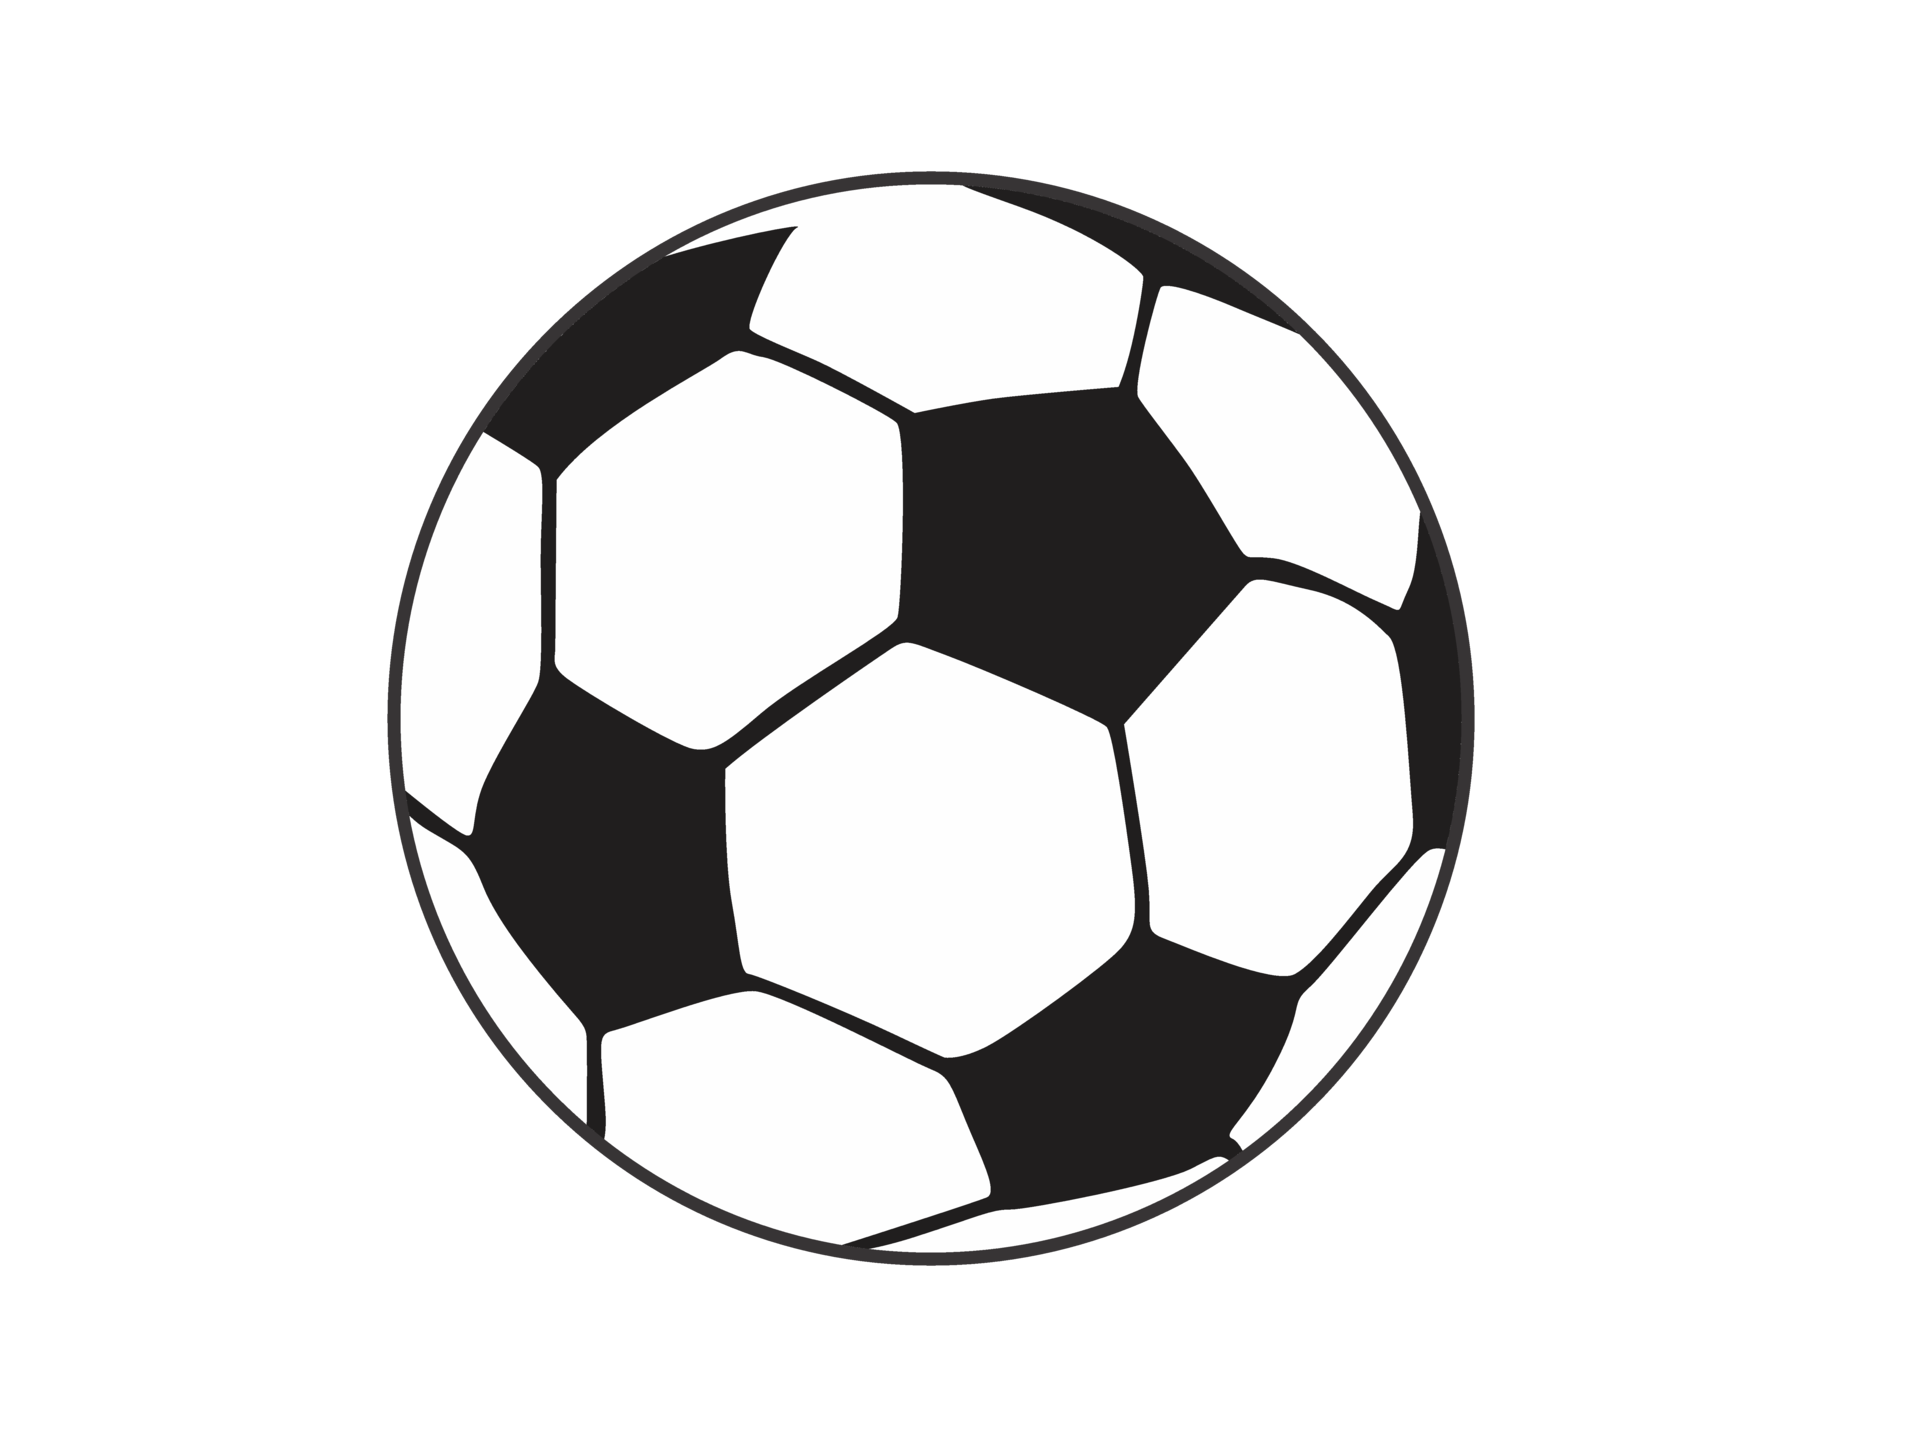
\includegraphics[scale=0.2]{Imagenes/IMG7/Pelota.png}
\end{center}

\end{document}